\documentclass[main.tex]{subfiles}
\begin{document}

\subsection{LQR}
\subsubsection{Definition}

The LQR is a control mechanism widely used in various fields, including aerospace, robotics, and industrial automation. It assumes that the system dynamics are linear and that the cost function is quadratic, which might not be applicable for highly nonlinear systems or those with complex constraints. LQR is used in a closed-loop-system to calculate the optimal feedback-gain \textit{K}, similarly to pole-placement.


The control-vector \textit{u} can be obtained as follows:
$$u(t) = -Kx(t)$$

\begin{figure}[h]
\centering
\resizebox{\linewidth}{!}{
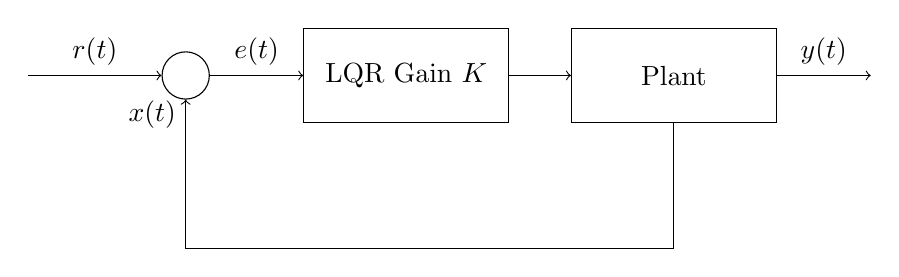
\begin{tikzpicture}[auto, node distance=2cm]

% Styles
\tikzstyle{block} = [draw, rectangle, minimum height=1.2cm, minimum width=2.6cm]
\tikzstyle{sum}   = [draw, circle, inner sep=0pt, minimum size=6mm]
\tikzstyle{input} = [coordinate]
\tikzstyle{output}= [coordinate]

% Nodes
\node [input, name=r] {};
\node [sum, right of=r] (sum1) {};
\node [block, right of=sum1, node distance=2.8cm] (lqr) {LQR Gain $K$};
\node [block, right of=lqr, node distance=3.4cm] (plant) {Plant};
\node [output, right of=plant, node distance=2.5cm] (y) {};

% Feedback coordinate
\node [coordinate, below of=plant, node distance=2.2cm] (fb_x) {};

% Forward path
\draw [->] (r) -- node {$r(t)$} (sum1);
\draw [->] (sum1) -- node {$e(t)$} (lqr);
\draw [->] (lqr) -- node {} (plant);
\draw [->] (plant) -- node {$y(t)$} (y);

% State feedback
\draw [->] (plant) -- (fb_x) -| node[pos=0.95, left] {$x(t)$} (sum1);

\end{tikzpicture}
}
\caption{LQR state-feedback control block diagram}
\label{fig:lqrblock}
\end{figure}


\subsubsection{Cost function}

What makes LQR so useful is the cost function used to determine how optimally the system behaves with respect to the state and the control-effort. It is calculated as follows:

$$J = \int_{0}^{\infty}{(x^TQx + u^TRu)}dt$$

where:
\begin{itemize}
    \item x is the \gls{state-vector},
    \item u is the \gls{control-vector},
    \item Q is a positive semi-definite $m \times m$ matrix that penalizes deviations in the state variables where \textit{m} is the number of states,
    \item R is a positive definite $n \times n$ matrix that penalizes the use of control-effort where \textit{n} is the number of inputs
\end{itemize}

The system is the most optimal when \textbf{J} is the lowest.

\subsubsection{Parameters}

Since \textit{Q} affects the state variable, increasing it leads to faster convergence, but higher control-effort. On the other hand, increasing \textit{R} slows down convergence and also decreases the effort. For example, this means that larger values of \textit{Q} would place the poles of the closed-loop-system matrix further left in the s-plane, resulting in the state decaying faster to zero.

\subsubsection{Continuous-time Algebraic Riccati Equation (CARE)}

An alternative to brute-forcing or using learning algorithms to find \textit{K}, the \textit{Riccati Equation} can be used to calculate the optimal feedback gain. It is derived from introducing a matrix \textit{P} such that $P=P^T$. The following matrix equation arises:


\begin{equation} \label{eq:2}
A^TP+PA+Q-PBR^{-1}B^TP = 0
\end{equation}

By substituting the control vector \textit{u} for $-Kx(t)$ and optimizing for $u$ we find that:

$$K = R^{-1}B^TP$$

Since equation \ref{eq:2} is linear, this simplifies the analysis and implementation. Because it is quadratic, the graphical representation of the cost map has a convex shape, thus it has a calculable global minimum.

\begin{figure}[hbt!]
    \centering
    \includegraphics[width=0.5\linewidth]{images/cost-map-ex.png}
    \caption{Example cost map}
    \label{fig:cost-map-ex}
\end{figure}

Picture \ref{fig:cost-map-ex} is simply an example of a graphical representation between \textit{J} and \textit{K}.

\subsubsection{Stability}
Similarly to the PID implementation, there were issues with computing the gains in Matlab, due to the initial instability of the system. To account for that the system was split in two subsystems. The first one is the electrical side of the system. It takes current as input and from its matrices we compute one gain $K_i$. We can think of it as an "inner" faster loop.
$$A_i = \frac{-R}{L_c}\ \  \ \ \  B_i = \frac{1}{L_c}\ \  \ \ \  x = i $$
$$ C_i = 1 \ \  \ \ \  Q_i = 1\ \  \ \ \   R_i = 1e-2$$
The outer loop takes care of the mechanical part and gives the other two gains $K_{o1/2}$.
$$A_o = \begin{bmatrix}
    0, 1 \\
    \frac{g}{l}, 0
\end{bmatrix} \ \  \ \ \ B_o = [0, \frac{2ki_0}{mld^2}]$$
$$C_o = [1,1]\ \  \ \ \ Q_o = \begin{bmatrix}
    100, 0 \\
    0, 1
\end{bmatrix} \ \  \ \ \ R_o = 1$$
 Together they are used to define the final gain matrix $K = [K_{o1}, K_{o2}, K_i]$.
Here is an example matlab script used to compute the gains and check of system stability using, the eigenvalues of the closed loop state matrix $A_{cl}$:
\begin{lstlisting}[
frame=single,
numbers=left,
style=Matlab-Pyglike]
%% Inner Loop 
Ai = -R/Lc;
Bi = 1/Lc;
Qi = 1;
Ri = 1e-2;
Ki = lqr(Ai, Bi, Qi, Ri);

%% Outer Loop
Ao = [0 1; g/l 0];
Bo = [0; alpha];
Qo = diag([100 1]);
Ro = 1;
Ko = lqr(Ao, Bo, Qo, Ro);

K = [Ko(1) Ko(2) Ki];

A = [ 0 1 0;g/l 0 alpha;0 0 -R/Lc ];
B = [0; 0; 1/Lc];

if all(real(eig(A-K*B)) >= 0)
    disp('SYSTEM IS UNSTABLE');
end
\end{lstlisting}
The system presented above is not guaranteed to be stable. If the $Q$ and $R$ values are changed or any of the parameters, it could cause the system to become unstable. To counter this, the $k$ coefficient should be adjusted accordingly. For this project it seems fit to penalize voltage control by reducing $R_i$ and increasing $Q_o(0,0)$ which controls $\phi$ to 0.01 and 100 respectively. The matlab result is as follows:
\begin{lstlisting}[
frame=single,
numbers=left,
style=Matlab-Pyglike]
Inner current gain Ki = 6.7703
Outer gains Ko = [10.9315 1.2634]

Closed-loop poles:
 1.0e+02 *
 -5.3425 + 0.0000i
 -0.0213 + 0.0004i
 -0.0213 - 0.0004i
\end{lstlisting}
 
\end{document}